\documentclass[dvipdfmx,a4paper,11pt]{article}
\usepackage[utf8]{inputenc}
%\usepackage[dvipdfmx]{hyperref} %リンクを有効にする
\usepackage{url} %同上
\usepackage{amsmath,amssymb} %もちろん
\usepackage{amsfonts,amsthm,mathtools} %もちろん
\usepackage{braket,physics} %あると便利なやつ
\usepackage{bm} %ラプラシアンで使った
\usepackage[top=20truemm,bottom=20truemm,left=20truemm,right=20truemm]{geometry} %余白設定
\usepackage{latexsym} %ごくたまに必要になる
\renewcommand{\kanjifamilydefault}{\gtdefault}
\usepackage{otf} %宗教上の理由でmin10が嫌いなので
%\usepackage{showkeys}\renewcommand*{\showkeyslabelformat}[1]{\fbox{\parbox{2cm}{ \normalfont\tiny\sffamily#1\vspace{6mm}}}}
\usepackage[driverfallback=dvipdfm]{hyperref}


\usepackage[all]{xy}
\usepackage{amsthm,amsmath,amssymb,comment}
\usepackage{amsmath}    % \UTF{00E6}\UTF{0095}°\UTF{00E5}\UTF{00AD}\UTF{00A6}\UTF{00E7}\UTF{0094}¨
\usepackage{amssymb}  
\usepackage{color}
\usepackage{amscd}
\usepackage{amsthm}  
\usepackage{wrapfig}
\usepackage{comment}	
\usepackage{graphicx}
\usepackage{setspace}
\usepackage{pxrubrica}
\usepackage{enumitem}
\usepackage{mathrsfs} 
\usepackage{caption}
\usepackage{ascmac}

\setstretch{1.2}


\newcommand{\R}{\mathbb{R}}
\newcommand{\Z}{\mathbb{Z}}
\newcommand{\Q}{\mathbb{Q}} 
\newcommand{\N}{\mathbb{N}}
\newcommand{\C}{\mathbb{C}} 
\newcommand{\Sin}{\text{Sin}^{-1}} 
\newcommand{\Cos}{\text{Cos}^{-1}} 
\newcommand{\Tan}{\text{Tan}^{-1}} 
\newcommand{\invsin}{\text{Sin}^{-1}} 
\newcommand{\invcos}{\text{Cos}^{-1}} 
\newcommand{\invtan}{\text{Tan}^{-1}} 
\newcommand{\Area}{\text{Area}}
\newcommand{\vol}{\text{Vol}}
\newcommand{\maru}[1]{\raise0.2ex\hbox{\textcircled{\tiny{#1}}}}
\newcommand{\sgn}{{\rm sgn}}
%\newcommand{\rank}{{\rm rank}}
\newcommand{\id}{{\rm id}}
\newcommand{\Sym}{{\rm Sym}}
\newcommand{\Supp}{{\rm Supp}}
\newcommand{\Ker}{{\rm Ker}}
\newcommand{\ima}{{\rm Im}}


\allowdisplaybreaks[4]
\usepackage{tcolorbox}
\tcbuselibrary{breakable, skins, theorems}

\theoremstyle{definition}
\newtheorem{thm}{定理}
\newtheorem{lem}[thm]{補題}
\newtheorem{prop}[thm]{命題}
\newtheorem{cor}[thm]{系}
\newtheorem{claim}[thm]{主張}
\newtheorem{dfn}[thm]{定義}
\newtheorem{rema}[thm]{注意}
\newtheorem{exa}[thm]{例}
\newtheorem{conj}[thm]{予想}
\newtheorem{prob}[thm]{問題}
\newtheorem{rem}[thm]{補足}

\DeclareMathOperator{\Ric}{Ric}
\DeclareMathOperator{\Vol}{Vol}
 \newcommand{\pdrv}[2]{\frac{\partial #1}{\partial #2}}
 \newcommand{\drv}[2]{\frac{d #1}{d#2}}
  \newcommand{\ppdrv}[3]{\frac{\partial #1}{\partial #2 \partial #3}}


\title{2025年度春夏学期 大阪大学 理学部数学科 \\ 幾何学基礎1演義 演習問題(基礎問題)}
\author{岩井雅崇 (大阪大学)}
\date{\today, \, ver 1.00}
%ここから本文.
\pagestyle{empty}

\begin{document}


\section{タイル1. }
\label{sec-tile1}
図1のようなチェス盤は, 図2のような2×1のタイルで埋め尽くすことができないことを示せ.

ただし2×1のタイルは重なり合ってはいけないしはみ出てはいけない.
\begin{figure}[htbp]
\begin{center}
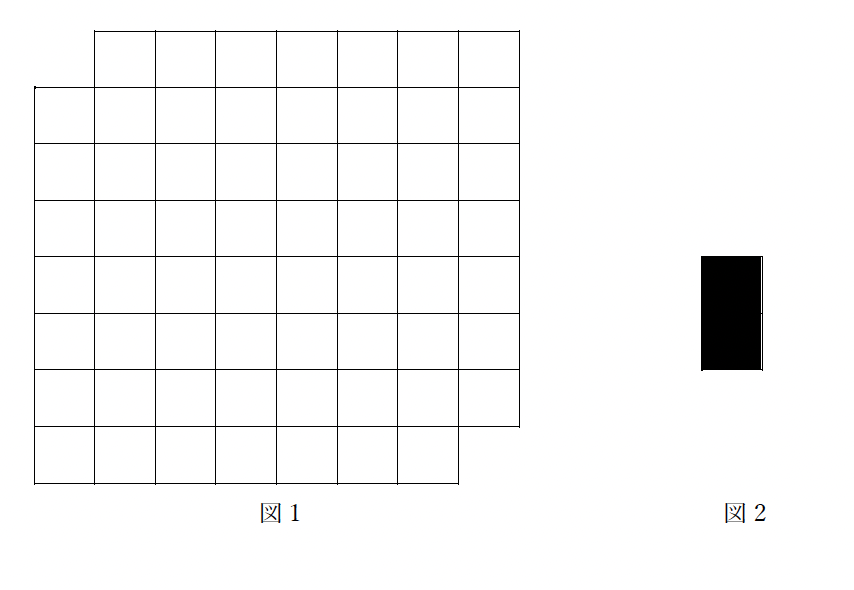
\includegraphics[width=60mm]{tile1.png}
\end{center}
\end{figure}


\section{タイル2. }
図1のような8×8のタイルの上に, 1×1タイルを好きなところにおく. 
このとき1×1タイルをどこにおいても, 図2のようなのタイルで埋め尽くすことができることを示せ.

ただし図2のようなタイルは重なり合ってはいけないしはみ出てはいけない.
\begin{figure}[htbp]
\begin{center}
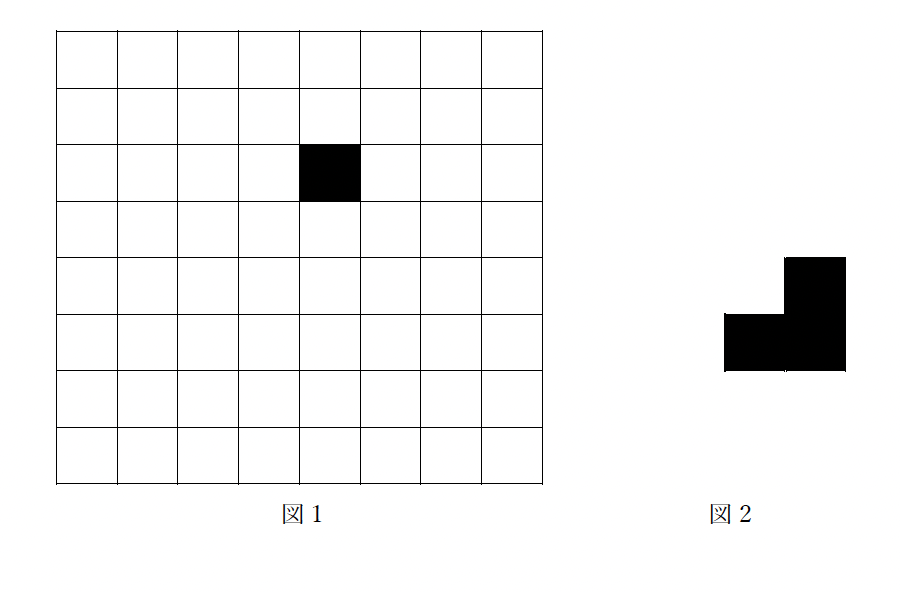
\includegraphics[width=60mm]{tile2.png}
\end{center}
\end{figure}

\section{タイル3. }
大きなタイルをたくさんの(有限個の)小さな長方形に分割した. 
その際全ての小さな長方形の縦の長さもしくは横の長さのどちらか(あるいは両方ともが)整数であった.

\vspace{5pt}
このとき, 大きな長方形の縦の長さもしくは横の長さのどちらか(あるいは両方とも)整数であることを示せ.
\begin{figure}[htbp]
\begin{center}
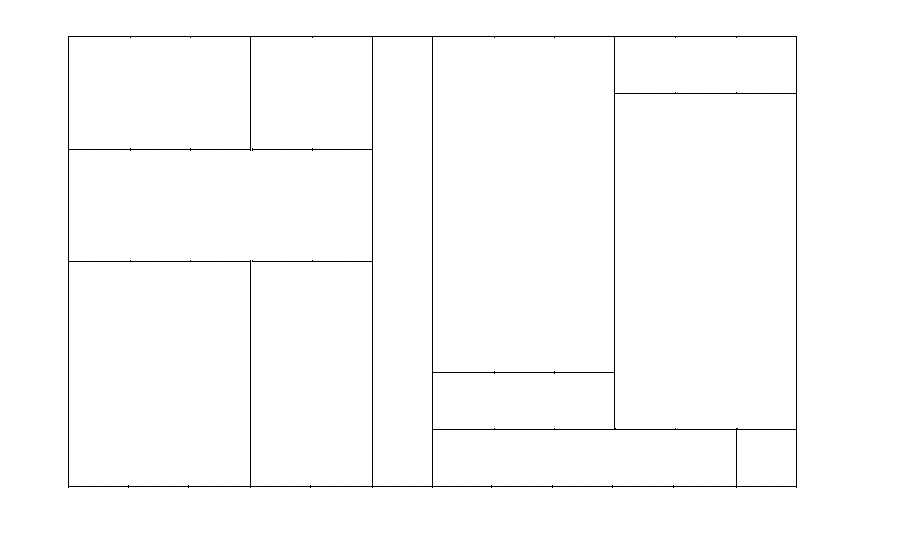
\includegraphics[width=70mm]{tile3.png}
\end{center}
\end{figure}


\newpage




\section{Kontsevichのパズル}
図1のようにタイルが無限に並んでいて, 左下のみ黒で他は白であるものを考える.
次の操作を何回やっても, 図2の赤色の部分に黒のタイルがあることを示せ. 

\vspace{5pt}
[操作] 図1のように上も右も白であるような黒のタイルを選び, それを白タイルに変えて, その上も右も黒のタイルに変える.

\begin{figure}[htbp]
\begin{center}
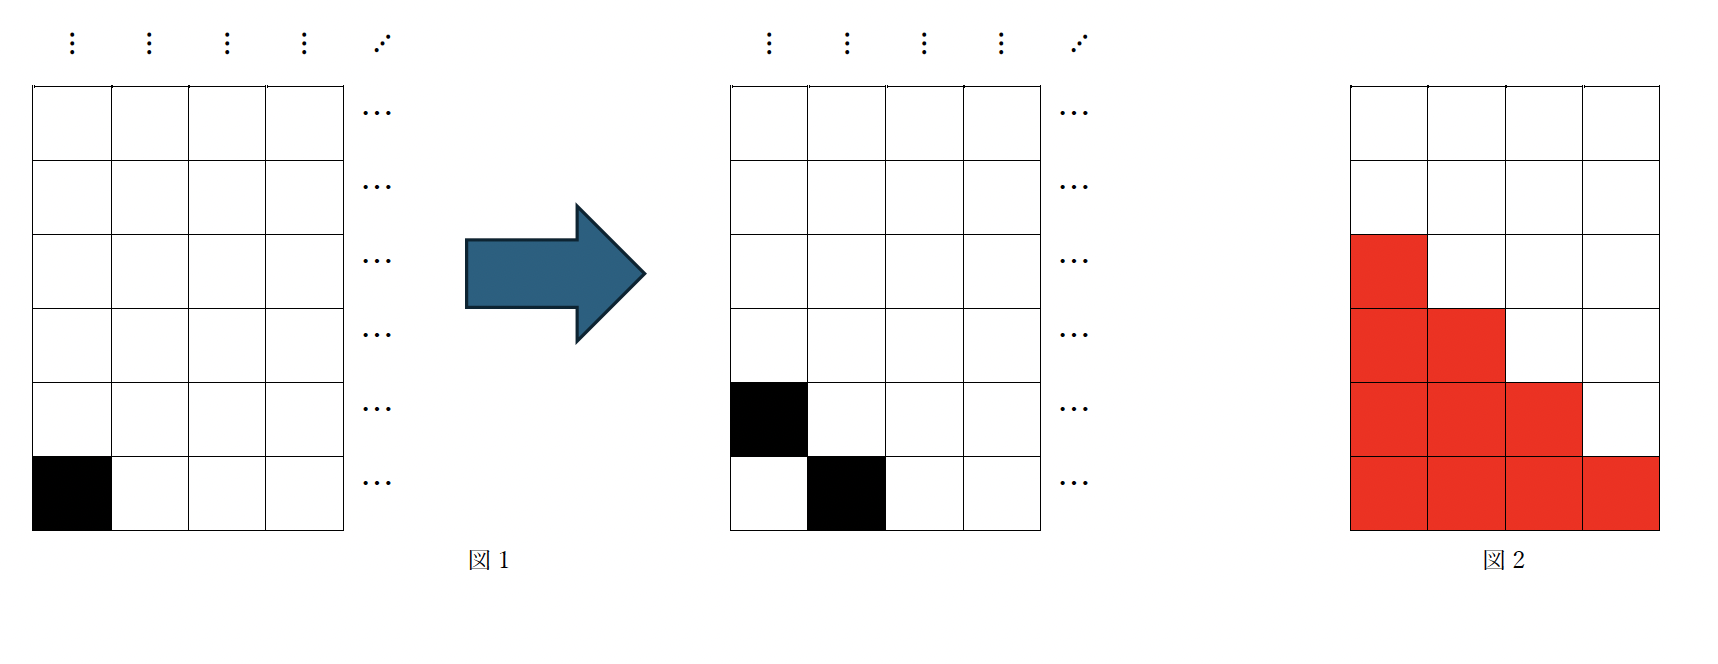
\includegraphics[width=100mm]{kont.png}
\end{center}
\end{figure}


\section{ドブル}
7色(赤, 橙, 黄, 緑, 青, 藍, 紫) のペンと7枚のカードある. 次のルールを考える.
\begin{enumerate}
    \setlength{\parskip}{0cm} 
  \setlength{\itemsep}{0cm} 
\item どのカードにも相異なる3 色の$\bullet$印がある.
\item どの2 枚のカードを取っても, 1 つだけ共通する色の$\bullet$印がある.
\end{enumerate}
上のルール2 つを満たすように色ペンを使ってカードに$\bullet$印を書くことはできるだろうか?

[補足] これをゲームにしたのがドブルである. ドブルで使うカードには, どんな2枚のカードを取っても共通する絵柄が必ず一つのみある. 

\section{11111.....}
$p$を2や5でない素数とする. 
$11111\cdots 111$という1が何個か並んだ形の$p$の倍数が存在することを示せ.

\vspace{10pt}
例えば...
\begin{itemize}
    \setlength{\parskip}{0cm} 
  \setlength{\itemsep}{0cm} 
  \item $p=3$の場合は111は3の倍数.
  \item $p=7$の場合は111111は7の倍数.
  \item $p=11$の場合は11は11の倍数.
  \end{itemize}
  
\section{2010年大阪大学理系第3問}
$l,m,n$を3以上の整数とする. 等式
$$
\left( \frac{n}{m} - \frac{n}{2} + 1 \right)l = 2
$$
を満たす$l,m,n$の組を全て求めよ. 

[補足] 実はこの方程式は隣の部屋の展示物と大きな関連がある. 



\section{コイン 1}
テーブル上に10個の硬貨が一列に並んでいる. 
その硬貨の額は1円か5円か10円である. 

あなたと私の二人で次のルールの下, 以下のゲームを行う.
\begin{itemize}
\item 列のうち左端か右端の硬貨を取る. その後次の人に手番をわたす.
\item とった硬貨の総額が多い方が勝ち. 同じであれば引き分け. 
\end{itemize}

ゲームに"負けたくない"あなたなら先手・後手どちらを選べば良いだろうか?
またその際どのような戦略を取れば良いだろうか?



\section{コイン 2}
テーブル上に25個の1円玉がある.
あなたと私の二人で次のルールの下, 以下のゲームを行う.

\begin{itemize}
\item テーブルの上の1円玉から, 1枚か2枚か3枚のコインを取る. その後次の人に手番をわたす.
\item 最後の1円玉を取った人が負け.
\end{itemize}

ゲームに"負けたくない"あなたなら先手・後手どちらを選べば良いだろうか?
またその際どのような戦略を取れば良いだろうか?


\section{コイン 2'}
テーブル上に25個の1円玉がある.
あなたと私の二人で次のルールの下, 以下のゲームを行う.

\begin{itemize}
\item テーブルの上の1円玉から, \underline{1枚か3枚か4枚}のコインを取る. その後次の人に手番をわたす.
\item 最後の1円玉を取った人が負け.
\end{itemize}


ゲームに"負けたくない"あなたなら先手・後手どちらを選べば良いだろうか?
またその際どのような戦略を取れば良いだろうか?

\section{コイン 3}
1円玉が表向きに$5 \times 5$の正方形に並んでいる.
次の操作を考える. 
\begin{itemize}
\item 縦か横に連続する3枚の1円玉を同時にひっくり返す.
\end{itemize}

 この操作を何回かして全ての1円玉を裏向きにできるか?

\section{$1 + \sqrt{2}$}
$(1 + \sqrt{2})^{2015}$の小数第100位を求めよ.





 \end{document}
